%doc: aulamobil/Aulamobil.doc
\begin{news}
{2} %columnes
{L'aulamòbil de les professions a l'escola!}
%index: L'aulamòbil de les professions
{El passat mes 21 d’octubre es va instal·lar a la nostra escola l’aula mòbil per a les professions destinada a l’alumnat de 4t d’ESO}
{ESO}
{11} %pagesof

\noindent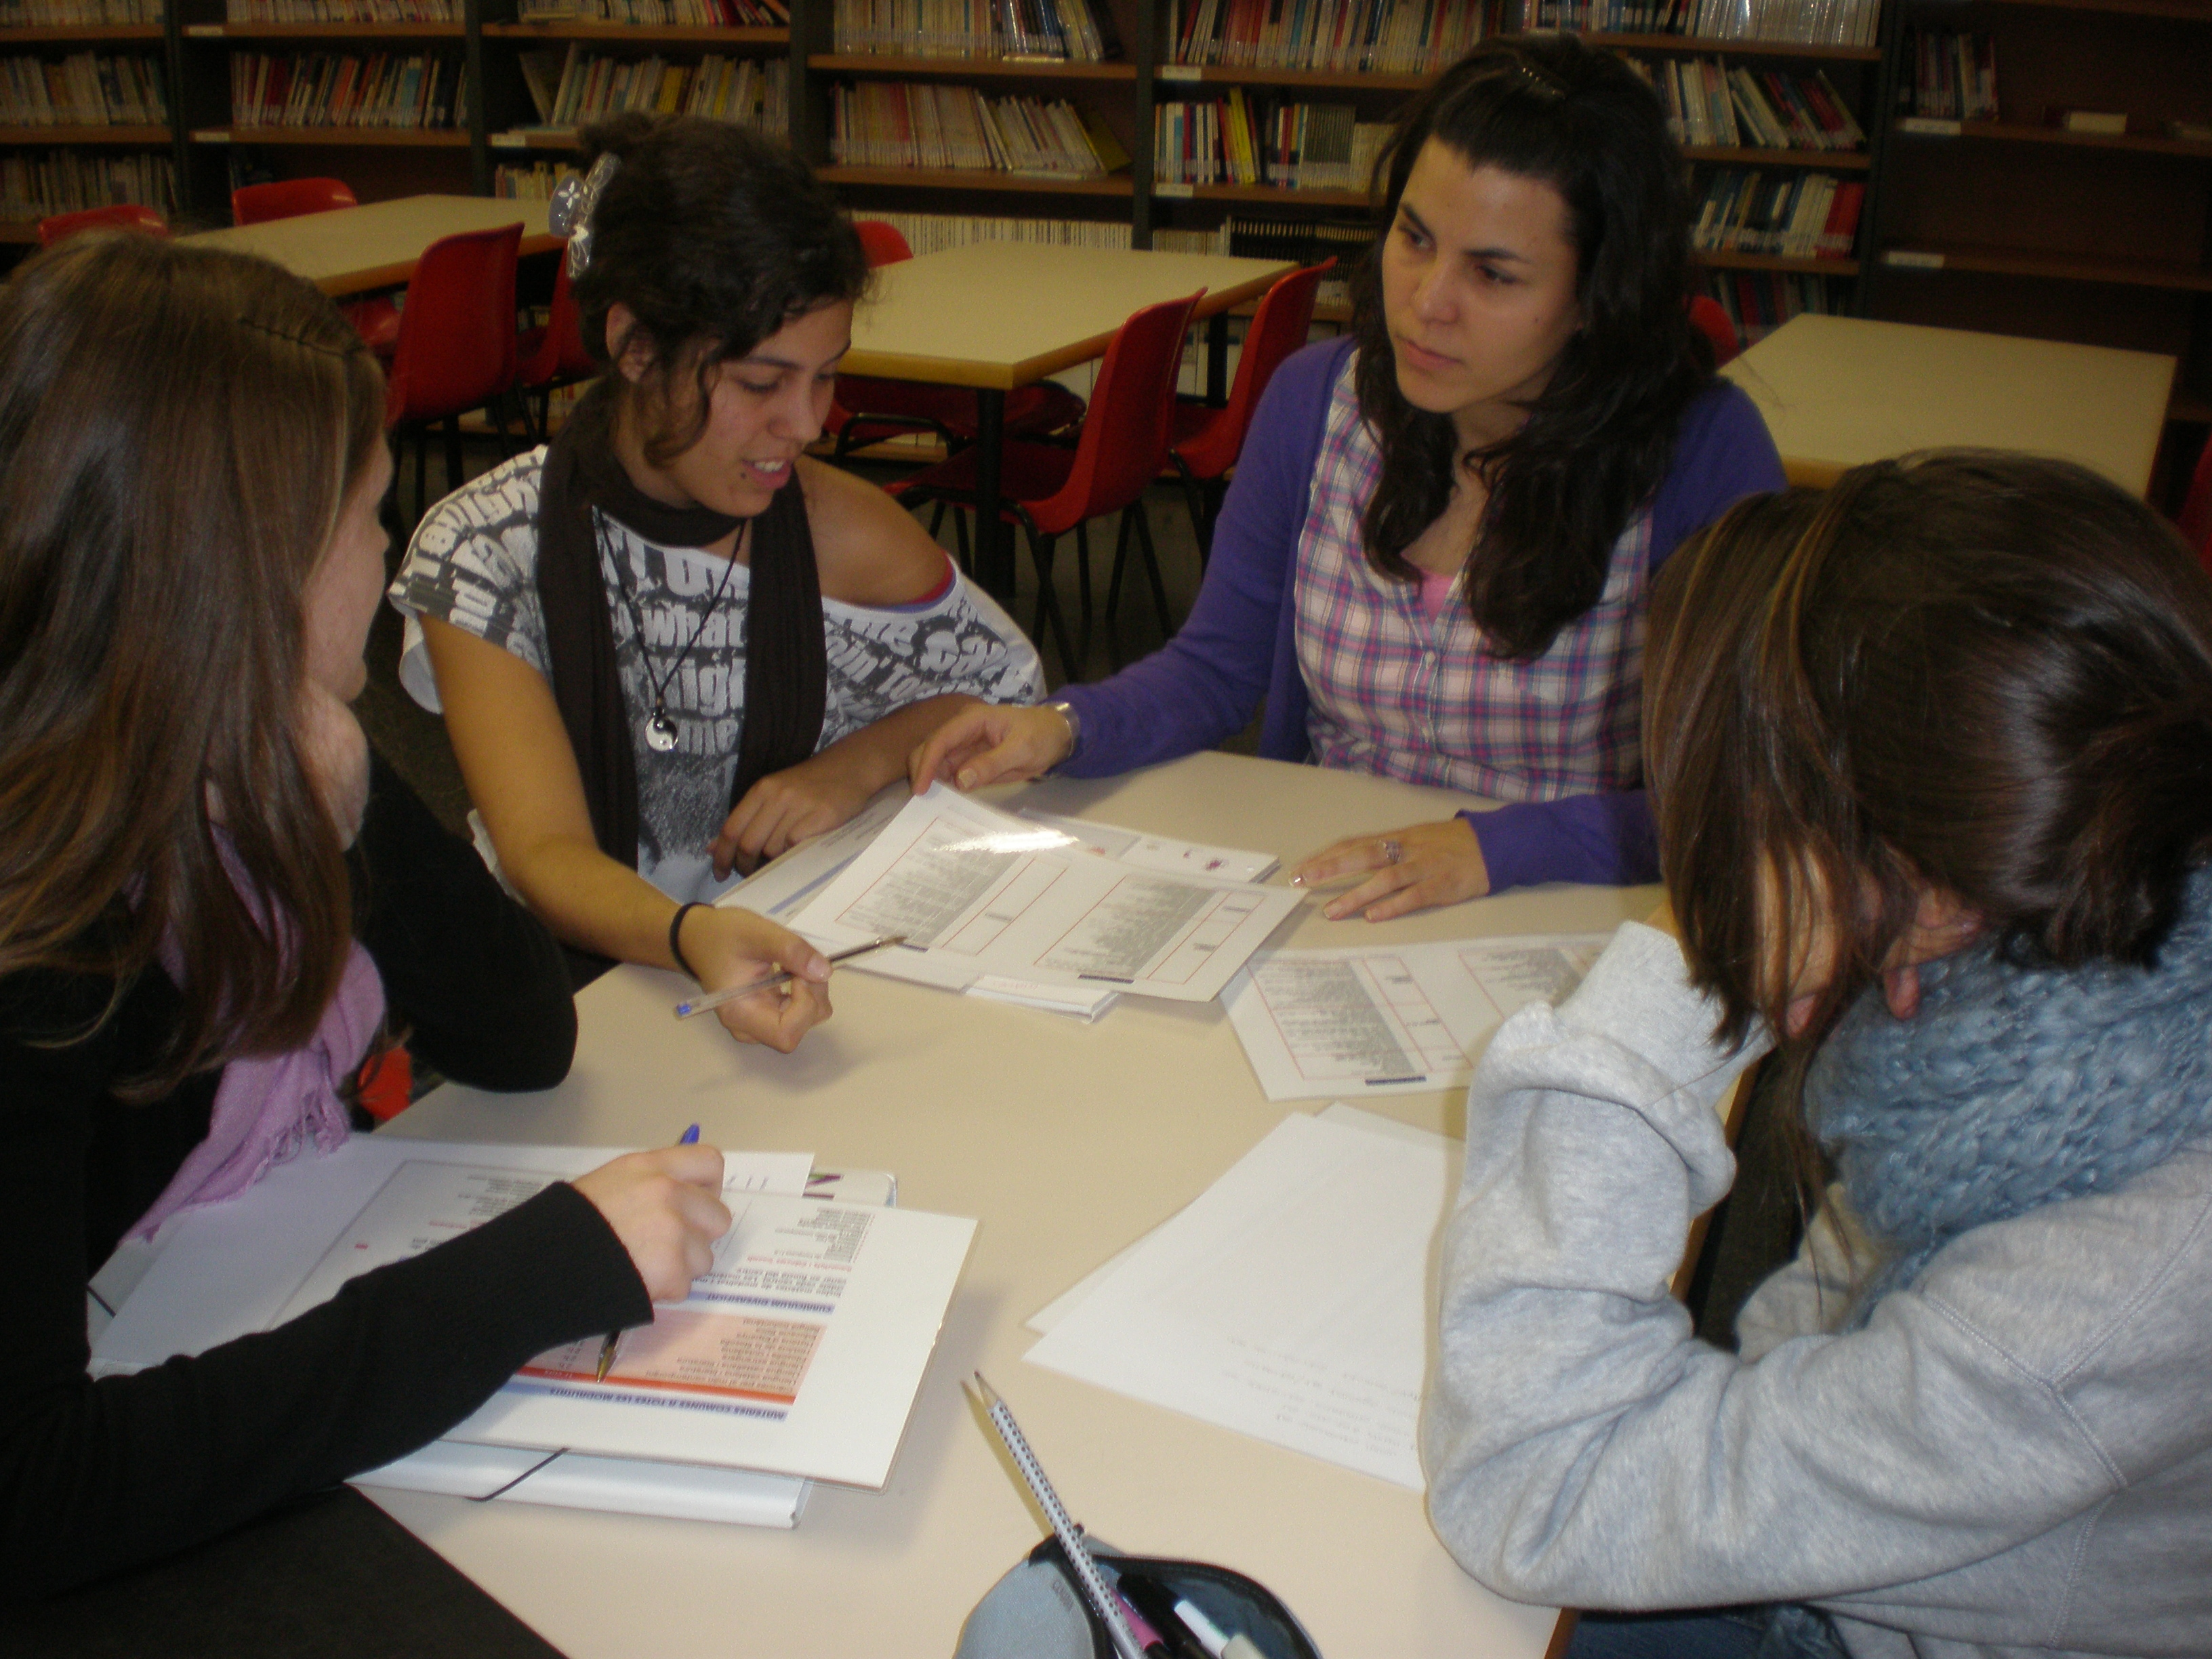
\includegraphics[width=9cm,keepaspectratio]{eso/img/Aulamobil3.JPG}

El passat mes 21 d’octubre es va instal·lar a la nostra escola l’aula mòbil per a les professions destinada a l’alumnat de 4t d’ESO.

Els nois i noies hi van trobar un enorme cabdal d’informació sobre els estudis que tenen al seu abast quan acabin l’ESO i les professions existents que s’hi relacionen.

Es van tractar temes com ara:

\begin{itemize}

	\item La formació professional. Els cicles formatius de grau mitjà: totes les especialitats, requisits d’accés, sortides professionals dels estudis, els centres de formació on s’imparteixen i l’accés posterior als de grau superior.

	\item El Batxillerat: les diferents modalitats i la correspondència amb la Universitat i amb la formació professional de grau superior.

	\item La Universitat. Les proves d’accés, les notes de tall, les noves carreres universitàries de l’espai europeu, les universitats i els centres adscrits, les passarel·les entre carreres, els plans d’estudi, etc.

	\item Els ensenyaments artístics i especialitzats. Els cicles formatius de grau mitjà d’arts plàstiques i disseny, el teatre, la dansa i la música

	\item Les sortides professionals corresponents a cada estudi i els perfils recomanats en cada ensenyament. 

\end{itemize}

\end{news}
